
\documentclass{beamer}


\usetheme{Frankfurt}
\usecolortheme{dove}
\usepackage{tikz}
\usetikzlibrary{arrows,shapes.arrows,positioning,shapes}
\usepackage{graphicx}
\usepackage{hyperref}
\newcommand\red[1]{{\color{red}#1}}
\newcommand\bred[1]{{\color{red}\textbf{#1}}}
\newcommand\blue[1]{{\color{blue}#1}}
\newcommand\bblue[1]{{\color{blue}\textbf{#1}}}
\newcommand\green[1]{{\color{olive}#1}}
\newcommand\bgreen[1]{{\color{olive}\textbf{#1}}}
\newcommand\black[1]{{\color{black}#1}}
\newcommand\white[1]{{\color{white}#1}}
\newcommand\gray[1]{{\color{darkgray}#1}}
\newcommand\E{\text{E}}
\newcommand\V{\text{V}}
\renewcommand\P{\text{P}}
\usepackage{soul}

\newcommand{\indep}{{\bot\negthickspace\negthickspace\bot}}

%%%%%%%%%%%%%%%%%%%%%%%%%%%%%%
\begin{document}

%\begin{frame}
%  \titlepage
%\end{frame}

\begin{frame}
\centering
\begin{tikzpicture}[x = .5\textwidth, y = .5\textheight]
\node[align = center, color = blue, font = \Large] at (0,.9) {A Research Note on the\\Prevalence of Housing Eviction\\Among Children Born in American Cities};
\node[align = center, font = \small] at (0, .52) {Ian Lundberg and Louis Donnelly\\Princeton University};
\node[align = center, font = \footnotesize] at (0, .25) {10 November 2018\\Fall Research Conference\\Association for Public Policy Analysis and Management};
\node[align = left, font = \tiny] at (0,-.25) {\begin{minipage}{.9\textwidth}Slides and source code are available at \blue{\url{https://github.com/ilundberg/slides}}. Replication code is available on the Harvard Dataverse: \blue{\url{https://doi.org/10.7910/DVN/BVWFG1}}. Draft is forthcoming in \emph{Demography}. Accepted manuscript is available \blue{\href{https://scholar.princeton.edu/sites/default/files/ilundberg/files/lundbergdonnelly2019_accepted.pdf}{here}}. We thank Sara S. McLanahan, Brandon M. Stewart, Matthew J. Salganik, three anonymous reviewers, and members of the Stewart Lab and the Fragile Families Working Group for comments on earlier drafts. All errors are our own. Research reported in this publication was supported by the Robert Wood Johnson Foundation and by The Eunice Kennedy Shriver National Institute of Child Health \& Human Development of the National Institutes of Health under Award Number P2CHD047879. Funding for the Fragile Families Study was provided through Award Numbers R01HD36916, R01HD39135, and R01HD40421 and by a consortium of private foundations. The content is solely the responsibility of the authors and does not necessarily represent the official views of the National Institutes of Health.\end{minipage}};
\end{tikzpicture}
\end{frame}

\section{Introduction}

\begin{frame}
%Eviction is a \bblue{traumatic experience} for families. \pause \vskip .5cm
\begin{center}
\begin{tikzpicture}[x = 1in, y = .4in]
\node at (-1,-3) {};
\node at (1,3) {};
\node[anchor = west] at (-1,1.4) {Eviction may play a role in the \bblue{reproduction of poverty}.};
\node (poverty) at (0,0) {Poverty};
\node (eviction) at (1,0) {Eviction};
\node[align=center] (poverty2) at (2,0) {More\\poverty};
\only<1-1,3->{\draw[->, thick] (poverty) -- (eviction);}
\only<2-2>{\draw[->, blue, line width = 2pt] (poverty) -- (eviction);}
\only<2-2>{\node[darkgray] at (1, -2) {Desmond, Gershonson, \& Kiviat 2015};}
\draw[->, thick] (poverty) to[bend right] (poverty2);
\only<1-2,4->{\draw[->, thick] (eviction) -- (poverty2);}
\only<3-3>{\draw[->, blue, line width = 2pt] (eviction) -- (poverty2);}
\only<3-3>{\node[darkgray, align = center] at (1, -2) {Desmond \& Kimbro 2015\\Desmond \& Shollenberger 2015};}
\only<5->{\node[anchor = west] at (-1,-2) {Yet policymakers largely \bblue{ignore this problem.}};}
\end{tikzpicture}
\end{center}
\end{frame}

\begin{frame}
Published studies suggest eviction is \bblue{rare in any given year}. \pause
\begin{itemize}
\item 0.3 \% of U.S. households in 12 months {\footnotesize \gray{(Bauman 2003)}} \pause
\item 2.3 \% in court records for 2016 {\footnotesize \gray{(Desmond et al. 2018)}} \pause
\end{itemize} \vskip .5cm
Eviction may be more common over the \bblue{course of childhood} \pause
\begin{itemize}
\item Families with children face a \bgreen{greater risk} {\footnotesize \gray{(Desmond et al. 2013)}} \pause
\item Risk \bgreen{accumulates} over time {\footnotesize \gray{(Duncan \& Rodgers 1988)}}
\end{itemize} \vskip .6cm \pause
\bblue{Research question:}
\begin{center}
What proportion of children born in large U.S. cities in 1998--2000\\
were \only<7-7>{ever evicted}\only<8-8>{\bgreen{ever evicted}} between birth and age 15?
\end{center}
%\begin{center}
%\begin{tabular}{rcccc}
%Bauman 2003 & 12 months in 1997--1998 & 0.3 \% \\
%Gould-Werth \& Seefeldt 2012 & 12 months in 2008--2010 in Detroit Metro Area &  2.4 \%
%%\end{tabular}
%\end{center}
\end{frame}

\begin{frame}

\includegraphics[width = \textwidth]{figures/ff_logo}
\begin{itemize}
\item Sampling frame: Births in 1998--2000 in U.S. cities with populations over 200,000
\item $N$ = 4,898 births in 20 cities
\begin{itemize}
\item 16 cities are a probability sample
\item 4 cities added for funder interests
\end{itemize}
\item Oversample (3:1) of non-marital births
\item Interviews with each parent at child age 1, 3, 5, 9, and 15
\end{itemize}
\end{frame}

\begin{frame}
\bblue{Survey instrument:}
\begin{center}
In the past 12 months, were you evicted from your home or apartment for not paying the rent or mortgage?
\end{center}
\begin{itemize}
\item[--] Reported by mother or father with whom child lives more than half the time
\end{itemize}
\end{frame}

\begin{frame}
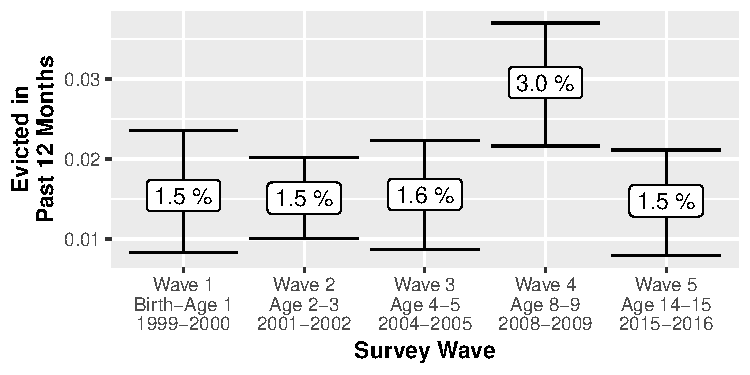
\includegraphics[width = \textwidth]{Output/evByWave_weightedOnly}
\end{frame}

\begin{frame}
\centering
\begin{tikzpicture}[x = .5\textwidth, y = .5\textheight]
\node at (-1,-1) {};
\node at (1,1) {};
\node[anchor = west] at (-1, .7) {Child ages covered by eviction reports};
\node at (0,0) {\includegraphics[width = \textwidth]{Output/evictionData_largeLabels}};
% Block out parts of figure I will highlight in other ways on slide
\draw[color = white, fill = white] (-1,0.2) rectangle (1,.4);
\draw[color = white, fill = white] (-1,0.02) rectangle (0,.12);
\draw[color = white, fill = white] (-1,-.08) rectangle (1,-.03);
\only<2-2>{
	\node (annual) at (0, .23) {12 months preceding each survey};
	\draw[line width = 1.5pt, blue, rounded corners] (-.9,.07) rectangle (.95,.32);
}
\only<3-3>{
	\node[align = center] at (0.5, .5) {Retrospective:\\Any eviction between\\ages 9 and 15};
	\draw[->, line width = 1.5pt, blue] (0.5, 0.3) -- (0.5, 0.07);
}
\only<4-4>{
	\node[align = center] at (-.38, .5) {Periods with no report};
	\draw[->, line width = 1.5pt, blue] (-.07, 0.45) -- (-.07, 0.15);
	\draw[->, line width = 1.5pt, blue] (-.43, 0.45) -- (-.43, 0.15);
	\draw[->, line width = 1.5pt, blue] (-.67, 0.45) -- (-.67, 0.15);
}
\only<5-5>{
\node at (0,.5) {\bblue{Goal:} Proportion evicted at any point};
\draw[|-|, blue, line width = 2pt] (-.85,.4) -- (.9, .4);
}
\end{tikzpicture}
\end{frame}

\begin{frame}
\includegraphics[width = \textwidth]{Output/evictionModels_largeLabels}
\end{frame}

\section{Lower Bound}

\begin{frame}
\bblue{Lower bound}: Assume
\begin{enumerate}
\item No evictions in periods with no report
\item No evictions when reports are missing
\end{enumerate} \vskip .8cm \pause
{\Large
\begin{align*}
\text{Lower bound} &= \frac{\text{\# ever report an eviction (weighted)}}{\text{\# in sample}} \\
\onslide<3->{&= \bblue{7.9 \%} \\
&\quad \text{(CI: 7.1--8.9 \%)}}
\end{align*}
}
\onslide<4->{
\includegraphics[width = \textwidth, trim = {0 280 0 45}, clip]{Output/evictionModels_largeLabels} \\
\includegraphics[width = \textwidth, trim = {0 0 0 323}, clip]{Output/evictionModels_largeLabels}
}
\end{frame}

\section{Multiply Imputed}

\begin{frame}
\bblue{Multiply imputed}: Assume
\begin{enumerate}
\item No evictions in periods with no report
\item \st{No evictions when reports are missing}
\begin{itemize}
\item Reports are missing at random given $\vec{X}$
\end{itemize}
\end{enumerate} \vskip .8cm \pause
{\Large
\begin{align*}
& \frac{\text{\# ever report an eviction (weighted, imputed)}}{\text{\# in sample}} \\
\onslide<3->{&= \bblue{9.2 \%} \\
&\quad \text{(CI: 7.3--11.1 \%)}}
\end{align*}
}
\onslide<4->{
\includegraphics[width = \textwidth, trim = {0 190 0 130}, clip]{Output/evictionModels_largeLabels} \\
\includegraphics[width = \textwidth, trim = {0 0 0 323}, clip]{Output/evictionModels_largeLabels}
}
\end{frame}

\section{Model-based}

\begin{frame}
\bblue{Model-based}: Assume
\begin{enumerate}
\item \st{No evictions in periods with no report}
\begin{itemize}
\item Evictions follow an assumed parametric model
\end{itemize}
\item \st{No evictions when reports are missing}
\begin{itemize}
\item Reports are missing at random given $\vec{X}$
\end{itemize}
\end{enumerate} \pause
\begin{tikzpicture}
\onslide<2->{
\node at (0,0) {\begin{minipage}{\textwidth}\begin{align*}
Y_{c\left[i\left[t\right]\right]} &\sim \text{Bernoulli}\left(\pi_{c\left[i\left[t\right]\right]}\right) \\
\\
\pi_{c\left[i\left[t\right]\right]} &= \text{logit}^{-1}\left(\eta_{c\left[i\left[t\right]\right]}\right) \\
\\
\eta_{c\left[i\left[t\right]\right]} &= \alpha + \vec{X}_{c\left[i\right]}\vec\beta + \text{Age}_{c\left[i\left[t\right]\right]}\gamma + \text{Recession}_{c\left[i\left[t\right]\right]}\lambda + \delta_c + \epsilon_{c\left[i\right]}
\end{align*}\end{minipage}};
}
\onslide<3-5>{
	\node[blue, font = \footnotesize] (stochastic) at (2,1) {Stochastic component};
	\draw[->, thick, blue] (stochastic.west) -- (-.6, 1);
	\node[blue, font = \footnotesize] at (-4.7,1.8) {Eviction};
	\draw[->, thick, blue] (-4.7, 1.6) -- (-4.7, 1.3);
	\node[blue, font = \footnotesize] at (-1.6,1.8) {$\P(\text{Eviction})$};
	\draw[->, thick, blue] (-1.6, 1.6) -- (-1.6, 1.2);
	\node[olive, font = \footnotesize] at (1.5,.3) (subscript) {Age $t$ for child $i$ born in city $c$};
	\draw[->, thick, olive] (subscript.west) to[out = 180, in = 320] (-4.5, .65);
	\draw[->, thick, olive] (subscript.west) to[out = 180, in = 270] (-1.3, .65);
}
\onslide<4-5>{
	% Linear predictor
	\node[blue, font = \footnotesize] (linear) at (1.5, -.9) {Linear predictor};
	\draw[->, blue, thick] (linear.west) to[out = 180, in = 0] (-1.8, -.9) to[out = 180, in = 270] (-2, -.6);
	\draw[->, blue, thick] (linear.west) to[out = 180, in = 0] (-1.8, -.9) to[out = 180, in = 90] (-4.7, -1.3);
}
\onslide<5-5>{
	% Equation
	\node[olive, font = \footnotesize, align = center] at (-2.7, -2.5) {Time-invariant\\predictors};
	\draw[->, olive, thick] (-2.7, -2.1) -- (-2.7, -1.8);
	\node[olive, font = \footnotesize, align = center] at (2, -2.7) {City\\random\\intercepts};
	\draw[->, olive, thick] (2.5, -2.5) -- (3.6, -1.8);
	\node[olive, font = \footnotesize, align = center] at (4.5, -2.7) {Individual\\random\\intercepts};
	\draw[->, olive, thick] (4.5, -2.1) -- (4.6, -1.8);
}
\onslide<6-6>{
	\node[olive, font = \footnotesize] at (-2.8, -2.25) {$\alpha \sim \text{Cauchy}(-4.5, 1)$};
	\node[olive, font = \footnotesize] at (.5, -2.25) {$\{\vec\beta,\gamma\lambda\}\sim \text{Cauchy}(0, 1)$};
	\node[olive, font = \footnotesize, align = center] at (4, -2.25) {$\delta_c\stackrel{\text{iid}}{\sim}\text{Normal}(0, \sigma^2_\delta)$};
	\node[olive, font = \footnotesize, align = center] at (4, -1) {$\epsilon_{c\left[i\right]}\stackrel{\text{iid}}{\sim}\text{Normal}(0, \sigma^2_\epsilon)$};
	\node[olive, font = \footnotesize, align = center] at (4, -3) {$\{\sigma^2_\delta,\sigma^2_\epsilon\}\stackrel{\text{iid}}{\sim}\text{Half-Cauchy}(0,1)$};
}
\end{tikzpicture}
\end{frame}

\begin{frame}
\begin{tikzpicture}[y = .4in]
\node at (0,1) {\begin{minipage}{\textwidth}\begin{align*}
Y_{c\left[i\left[t\right]\right]} &\sim \text{Bernoulli}\left(\pi_{c\left[i\left[t\right]\right]}\right) \\
\pi_{c\left[i\left[t\right]\right]} &= \text{logit}^{-1}\left(\eta_{c\left[i\left[t\right]\right]}\right) \\
\eta_{c\left[i\left[t\right]\right]} &= \alpha + \vec{X}_{c\left[i\right]}\vec\beta + \text{Age}_{c\left[i\left[t\right]\right]}\gamma + \text{Recession}_{c\left[i\left[t\right]\right]}\lambda + \delta_c + \epsilon_{c\left[i\right]}
\end{align*}\end{minipage}};
\onslide<2->{
\node at (-4,-.5) {\bblue{Procedure}};
}
\onslide<3->{
\node[anchor = west] at (-4.8,-1) {1. Draw parameters from posterior distribution: $\hat\alpha,\hat{\vec\beta},\hat\gamma,\hat\lambda,\hat\delta_c,\hat\epsilon_{c\left[i\right]}$};
}
\onslide<4->{
\node[anchor = west] at (-4.8,-1.6) {2. Transform to $\hat\pi_{c\left[i\left[t\right]\right]}$ at Age = $1,\dots,15$};
}
\onslide<5->{
\node[anchor = west] at (-4.8,-2.3) {3. Collapse across years};
\only<5>{
	\node at (0, -2.9) {$\hat\phi_{c\left[i\right]} = \P\left(\left[\text{Ever evicted}\right]_{c\left[i\right]}\right) = 1 - \prod_{t=1}^{15} \left(1 - \hat\pi_{c\left[i\left[t\right]\right]}\right)$};
}
\only<6>{
	\node at (0, -2.9) {$\hat\phi_{c\left[i\right]} = \P\left(\left[\text{Ever evicted}\right]_{c\left[i\right]}\right) = 1 - \prod_{t=1}^{15} \left(1 - \blue{\hat\pi_{c\left[i\left[t\right]\right]}}\right)$};
	\node[blue, font = \tiny] at (3.5, -2.3) {$\P(\text{Evicted at age }t)$};
	\draw[->, thick, blue] (3.5, -2.4) -- (3.5, -2.65);
}
\only<7>{
	\node at (0, -2.9) {$\hat\phi_{c\left[i\right]} = \P\left(\left[\text{Ever evicted}\right]_{c\left[i\right]}\right) = 1 - \prod_{t=1}^{15} \blue{\left(1 - \hat\pi_{c\left[i\left[t\right]\right]}\right)}$};
	\node[blue, font = \tiny] at (3.3, -2.3) {$\P(\text{\emph{Not} evicted at age }t)$};
	\draw[->, thick, blue] (3.3, -2.4) -- (3.3, -2.65);
}
\only<8>{
	\node at (0, -2.9) {$\hat\phi_{c\left[i\right]} = \P\left(\left[\text{Ever evicted}\right]_{c\left[i\right]}\right) = 1 - \blue{\prod_{t=1}^{15} \left(1 - \hat\pi_{c\left[i\left[t\right]\right]}\right)}$};
	\node[blue, font = \tiny] at (2.4, -2.3) {$\P(\text{\emph{Never} evicted by age 15})$};
	\draw[->, thick, blue] (2.4, -2.4) -- (2.4, -2.65);
}
\only<9>{
	\node at (0, -2.9) {$\blue{\hat\phi_{c\left[i\right]}} = \P\left(\left[\text{Ever evicted}\right]_{c\left[i\right]}\right) = \blue{1 - \prod_{t=1}^{15} \left(1 - \hat\pi_{c\left[i\left[t\right]\right]}\right)}$};
	\node[blue, font = \tiny] at (2.2, -2.3) {$\P(\text{\emph{Ever} evicted by age 15})$};
	\draw[->, thick, blue] (2.2, -2.4) -- (2.2, -2.65);
}
\only<10->{
	\node at (0, -2.9) {$\hat\phi_{c\left[i\right]} = \P\left(\left[\text{Ever evicted}\right]_{c\left[i\right]}\right) = 1 - \prod_{t=1}^{15} \left(1 - \hat\pi_{c\left[i\left[t\right]\right]}\right)$};
}
}
\onslide<10->{
\node[anchor = west] at (-4.8,-3.5) {4. Collapse across children};
\node at (0, -4.1) {Overall prevalence = $\hat\tau = \frac{\sum_{c=1}^{16}\sum_{i=1}^{n_c}w_{c\left[i\right]}\hat\phi_{c\left[i\right]}}{\sum_{c=1}^{16}\sum_{i=1}^{n_c}w_{c\left[i\right]}}$};
}
\onslide<11->{
\node[anchor = west] at (-4.8,-4.7) {5. Repeat for 10,000+ posterior draws of $\hat\tau$};
}
\onslide<12->{
\node[anchor = west, font = \Large] at (-5,-5.7) {\bblue{Result}: $\hat\tau_\text{PM} = 14.8$ \% (CI: 12.6--17.2 \%)};
}
\end{tikzpicture}
\end{frame}

\begin{frame}
\includegraphics[width = \textwidth]{Output/evictionModels_largeLabels}
\end{frame}

\section{Subgroups}

\begin{frame}
\centering \Large
Given our model, we can aggregate across the covariate values of specific \bblue{subgroups}.
\end{frame}

\begin{frame}
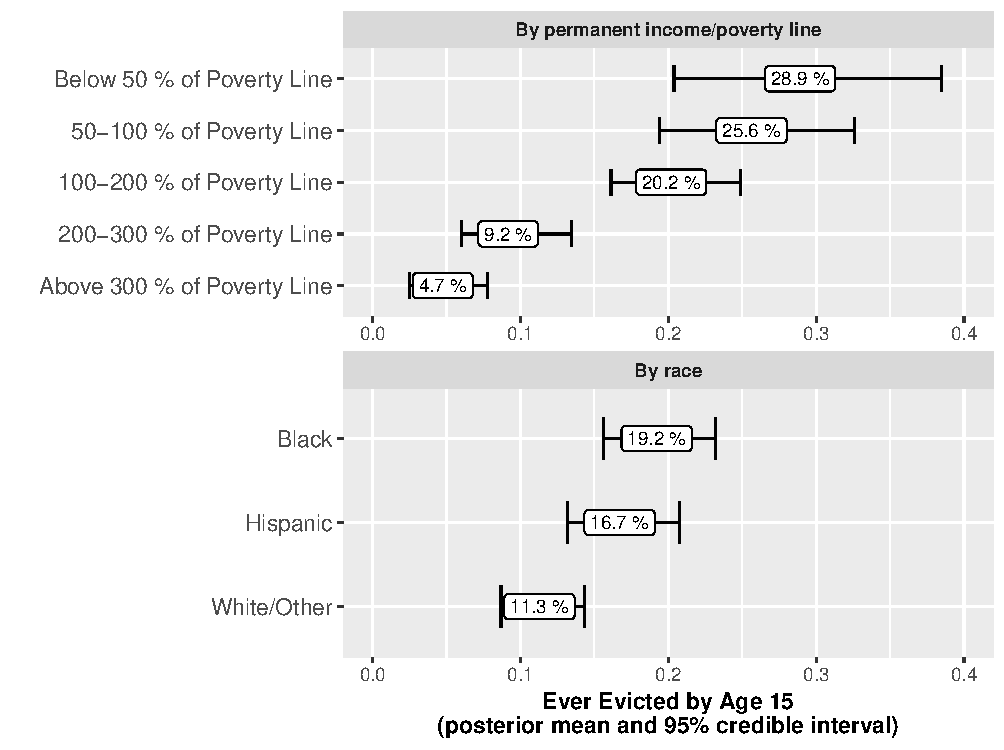
\includegraphics[width = \textwidth]{Output/RaceIncomeGroups_largeFont}
\end{frame}

\begin{frame}
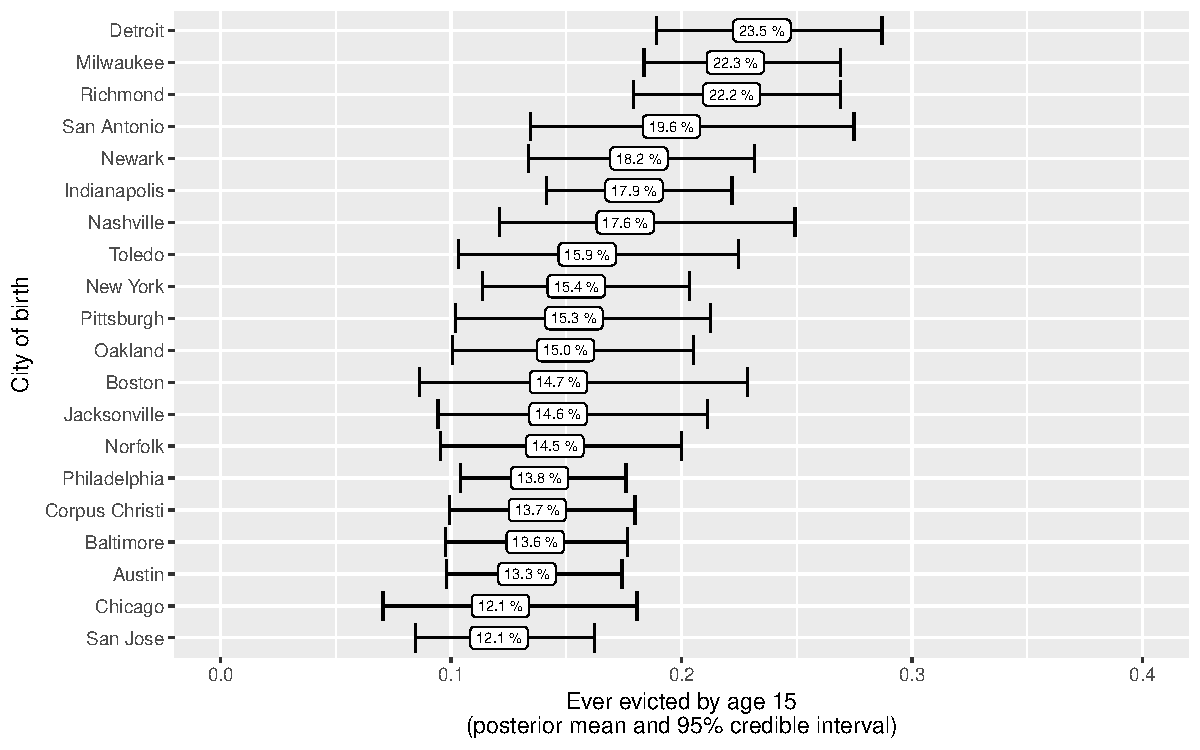
\includegraphics[width = \textwidth]{Output/ByCity}
\end{frame}

\section{Limitations}

\begin{frame}{Limitations}
\begin{itemize}
\item Attrition may be non-ignorable \pause
\begin{itemize}
\item[$\rightarrow$] we will underestimate eviction
\end{itemize} \pause
\item Self-report may understate eviction \pause 
\begin{itemize}
\item[$\rightarrow$] we will underestimate eviction \pause
\end{itemize}
\item Parametric model may be wrong \pause
\begin{itemize}
\item[$\rightarrow$] implication unclear, but robust to random forest
\end{itemize}
\end{itemize}
\end{frame}

\section{Conclusion}

\begin{frame}{Conclusion}
Eviction is 
\begin{itemize}
\item a \bblue{common} experience
\begin{itemize}
\item 1 in 7 children born in large U.S. cities in 1998--2000 were evicted by age 15
\end{itemize}
\item a \bblue{stratified} experience
\begin{itemize}
\item 1 in 4 among those born into deep poverty
\end{itemize}
\end{itemize}
\begin{center}
Policymakers should be concerned about the prevalence of eviction.
\end{center}
\end{frame}



\end{document}